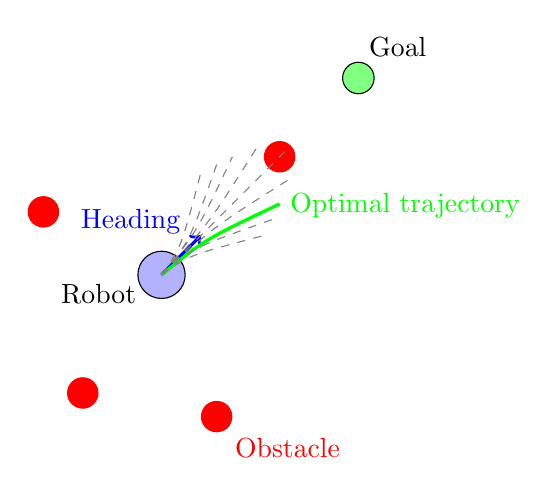
\begin{tikzpicture}

    % Robot
    \draw[fill=blue!30] (0, 0) circle [radius=0.3] node[anchor=north east, xshift=-0.2cm] {Robot};
    
    % Obstacles
    \fill[red] (1.5, 1.5) circle [radius=0.2];
    \fill[red] (-1.5, 0.8) circle [radius=0.2];
    \fill[red] (0.7, -1.8) circle [radius=0.2] node[xshift=0.9cm, yshift=-0.40cm] {Obstacle};
    \fill[red] (-1.0, -1.5) circle [radius=0.2];
    
    % Goal
    \draw[fill=green!50] (2.5, 2.5) circle [radius=0.2] node[xshift=0.5cm, yshift=0.4cm] {Goal};
    
    % Coordinate grid
    %\draw[->, thin, gray] (-3, 0) -- (3, 0) node[right] {$x$};
    %\draw[->, thin, gray] (0, -3) -- (0, 3) node[above] {$y$};
    
    % Heading
    \draw[->, very thick, blue] (0, 0) -- (0.5, 0.5) node[near end, left, yshift=0.3cm] {Heading};
    
    % Possible trajectories
    \draw[dashed, gray] (0, 0) .. controls (0.8, 0.8) .. (1.6, 1.6);
    
    \draw[dashed, gray] (0, 0) .. controls (0.60, 0.65) .. (1.2, 1.6);
    \draw[dashed, gray] (0, 0) .. controls (0.65, 0.60) .. (1.6, 1.2);

    \draw[dashed, gray] (0, 0) .. controls (0.45, 0.55) .. (0.9, 1.5);
    % Chosen trajectory
    \draw[very thick, green] (0, 0) .. controls (0.55, 0.45) .. (1.5, 0.9) node[near end, xshift=2.15cm, yshift=0.25cm] {Optimal trajectory};
    
    \draw[dashed, gray] (0, 0) .. controls (0.35, 0.41) .. (0.7, 1.4);
    \draw[dashed, gray] (0, 0) .. controls (0.41, 0.35) .. (1.4, 0.7);
    
    \draw[dashed, gray] (0, 0) .. controls (0.25, 0.35) .. (0.5, 1.3);
    \draw[dashed, gray] (0, 0) .. controls (0.35, 0.25) .. (1.3, 0.5);
    
    % Labels
    %\node[align=center] at (-2.5, -2.5) {\small Dynamic Window\\ \small of Velocities};
    %\draw[dotted, thick, ->] (-2, -2.0) -- (-1, -1);

\end{tikzpicture}